\section{Using the \Wilds package}\label{sec:library}
Finally, we discuss our open-source PyTorch-based package that exposes a simple interface to our datasets and automatically handles data downloads, allowing users to get started on a \Wilds dataset in just a few lines of code.
In addition, the package provides various data loaders and utilities surrounding domain annotations and other metadata, which supports training algorithms that need access to these metadata.
The package also provides standardized evaluations for each dataset.
More documentation and installation information can be found at \url{https://wilds.stanford.edu}.

\paragraph{Datasets and data loading.}
The \Wilds package provides a simple, standardized interface for all datasets in the benchmark as well as their data loaders, as summarized in \reffig{data_snippet}.
This short code snippet covers all of the steps of getting started with a \Wilds dataset, including dataset download and initialization, accessing various splits, and initializing the data loader.
We also provide multiple data loaders in order to accommodate a wide array of algorithms, which often require specific data loading schemes.
\begin{figure}[h]
  \centering
  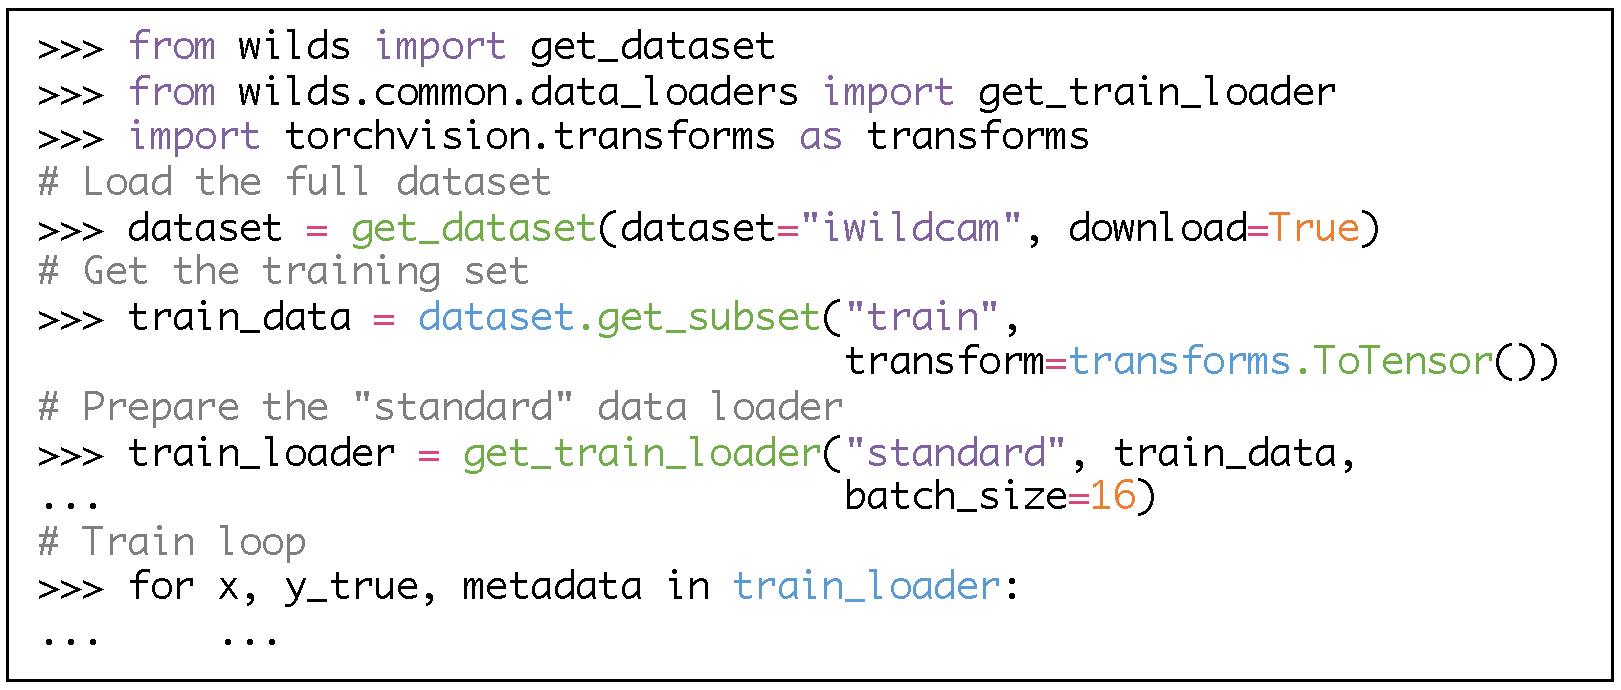
\includegraphics[width=0.8\linewidth]{figures/data_snippet.pdf}
  \caption{
    Dataset initialization and data loading.
    }
  \label{fig:data_snippet}
\end{figure}

\paragraph{Domain information.}
To allow algorithms to leverage domain annotations as well as other groupings over the available metadata, the \Wilds package provides \texttt{Grouper} objects.
\texttt{Grouper} objects (e.g., \texttt{grouper} in \reffig{grouper_snippet}) extract group annotations from metadata, allowing users to specify the grouping scheme in a flexible fashion.
\begin{figure}[h]
  \centering
  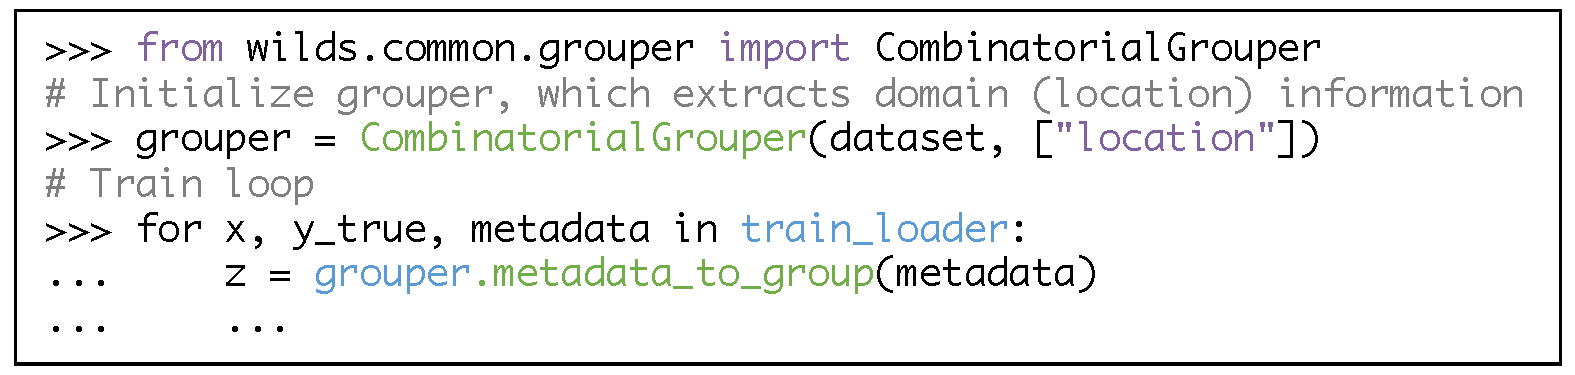
\includegraphics[width=0.8\linewidth]{figures/grouper_snippet.pdf}
  \caption{
    Accessing domain and other group information via a Grouper object.
    }
  \label{fig:grouper_snippet}
\end{figure}

\paragraph{Evaluation.}
Finally, the \Wilds package standardizes and automates the evaluation for each dataset.
As summarized in \reffig{eval_snippet}, invoking the \texttt{eval} method of each dataset yields all metrics reported in the paper and on the leaderboard.
\begin{figure}[h]
  \centering
  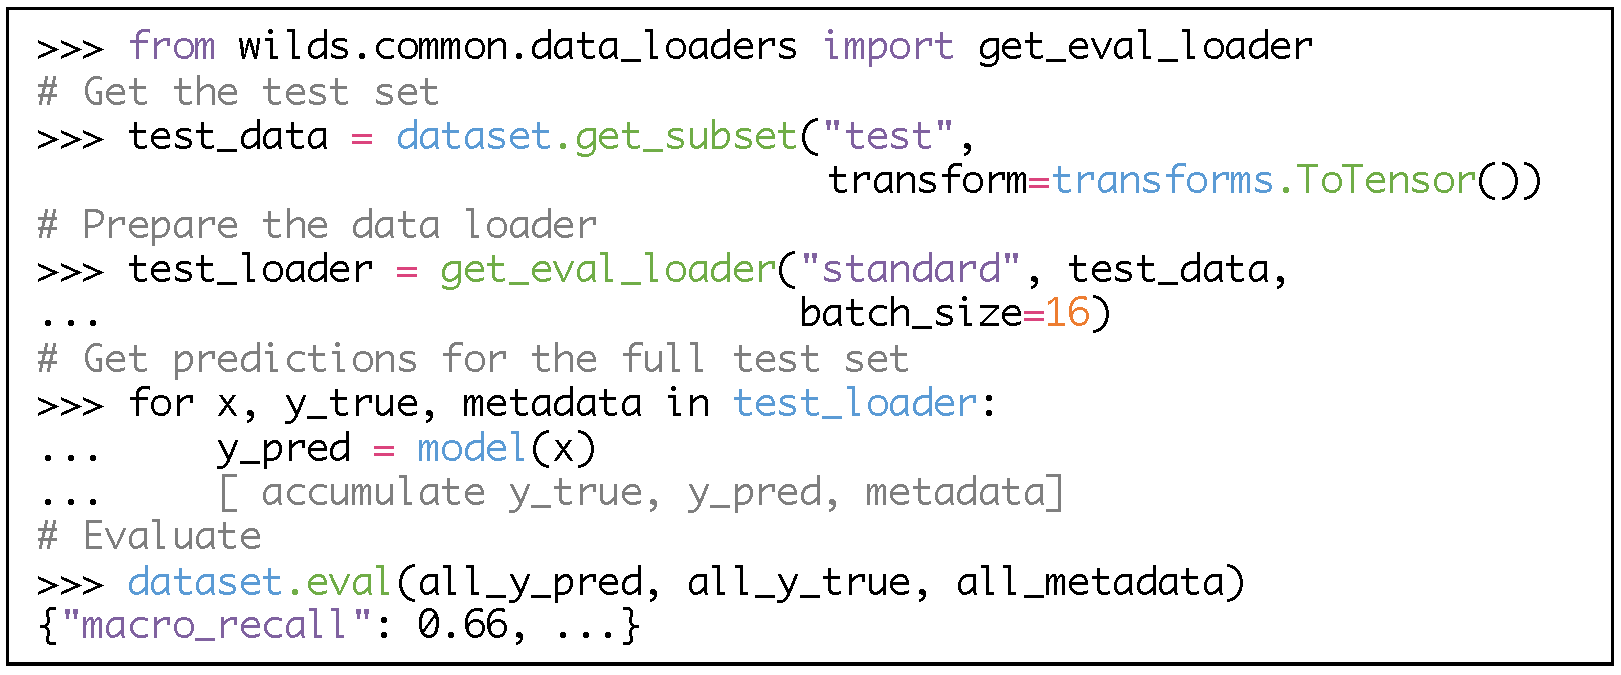
\includegraphics[width=0.8\linewidth]{figures/eval_snippet.pdf}
  \caption{
    Evaluation.
    }
  \label{fig:eval_snippet}
\end{figure}
